\subsection{Design Goal}
The purpose of building Least Privilege CTF is to effectively teach developers about how IAM works and how to adopt PoLP in GCP. Meanwhile, the CTFs should be able to run at minimum cost and fast, deliver instant feedback, extensible, friendly to beginners and scaffolding.
\begin{enumerate}
\item Minimum cost: Anyone can apply for 300 credits(dollars) for free with a Google account and credit card. If levels are deleted upon completion, monthly cost would be less than a dollar (Figure~\ref{fig:cost}). 
\begin{figure}[!h]
  \centering
  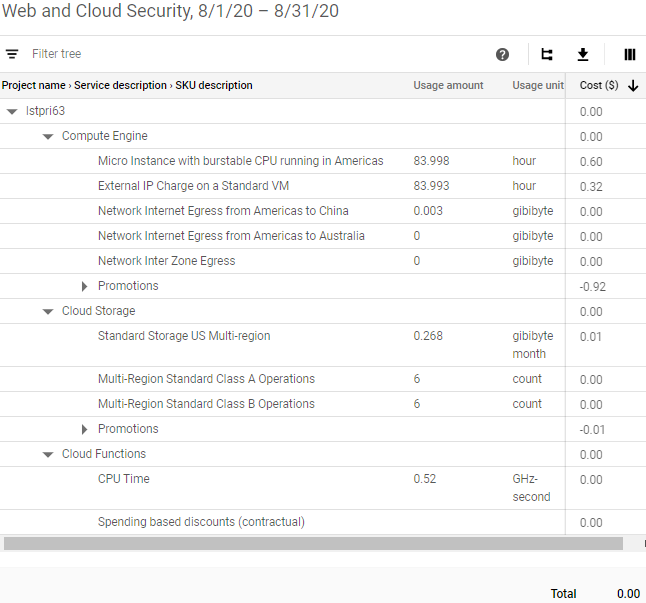
\includegraphics[width=\linewidth]{pic/cost}
  \caption {Billing - Monthly Cost}
  \label{fig:cost}
\end{figure}
\item Fast Deployment:  Deploy initial 11 levels in 4.5 minutes.
\item Extensible: Easy to add new level with simple modification. 
\item Beginners friendly: Explicit and detailed instructions are available in the UI for every level. Prior Google Cloud knowledge is optional.
\item Instant feedback: Results will show up immediately along with failing reason for each attempt.
\item Scaffolding: Differentiated and incremented level difficulties for the benefit of both novices and experienced practitioners.

\end{enumerate}

\subsection{Implementation}

\subsubsection{Thunder CTF and Modular}
Least privilege CTF is developed based on Thunder CTF, a scaffolded, scenario-based CTF that helps students learn about and practice cloud security skills on GCP. Each Thunder CTF level includes a yaml development configuration, a python deployment script and an HTML content for hints \cite{Springer}. The modular design and specific structure reduces the process of adding new levels to simply filling in a template. Least privilege CTF inherits the modular structure from Thunder CTF with modification. Rather than deploy each level individually, Least Privileges CTF deploys all required resources specified in the yaml file at one time in parallel with Google Cloud Deployment Manager, which takes about 4.5 mins for 11 levels.

\subsubsection{UI and Cloud Functions}
Despite a page \cite{lst-ctf} hosted under main Thunder CTF website for steps of environment set-up and initial deployment, Least Privilege CTF does not generate level hints with HTML contents or render scripts in a similar way as in Thunder CTF. Instead, the hints system is replaced by Cloud Function \cite{cloudfunc}, a pay-as-you-go service that automatically scales based on loads. There are several advantages comes from Cloud Function. First, services only get billed for execution time. Second, Cloud Functions demand no server management which speeds up the development as we do not have to deal with the operational infrastructure in Google Cloud. Third, Cloud Function integrates with logging and debugging capabilities, making the coding experience intuitive. Last, the service has built-in security based on PoLP at role per function. 

The type of function to create level instructions and hints in Least Privilege CTF is HTTP function. HTTP functions are invoked by standard HTTP requests and supports common methods like GET, PUT, POST, DELETE and OPTIONS \cite{httpfunc}. A typical procedure in our design framework is that when a function is triggered by events, it waits for responses either returned from a Cloud service or submitted in front-end using POST or GET method. Thanks to the TLS certificates that automatically provisioned in Cloud Functions service, all HTTP functions can be invoked with a secure connection. 

In order to call a function and pass parameters, an URL known as HTTP-Triggered-Endpoint is obtained after each function deployment. Figure~\ref{fig:endpoints} shows the function endpoints printed in Cloud Console shell when deployment manager completes the operation and creates initial levels. In Least Privilege CTF, functions are written in python and interact with other cloud services through APIs. The returned results of a function will be rendered into HTML through Jinja and appear in the form of a web page. Players can access the page in web browser via related function endpoint.

Each level contains two functions, an access function (Figure~\ref{fig:access}) and a check function (Figure~\ref{fig:check}). In the UI created with access function, players can find level resources, step by step instructions towards completion and a code snippet that helps figure out what the function does. The check function lists current roles and permissions that a player choose as the answer and displays the validation result. In addition,  a Scoreboard Function is implemented to keep track of the overall accomplishment of all levels (Figure~\ref{fig:score}).  
\begin{figure}[!h]
  \centering
  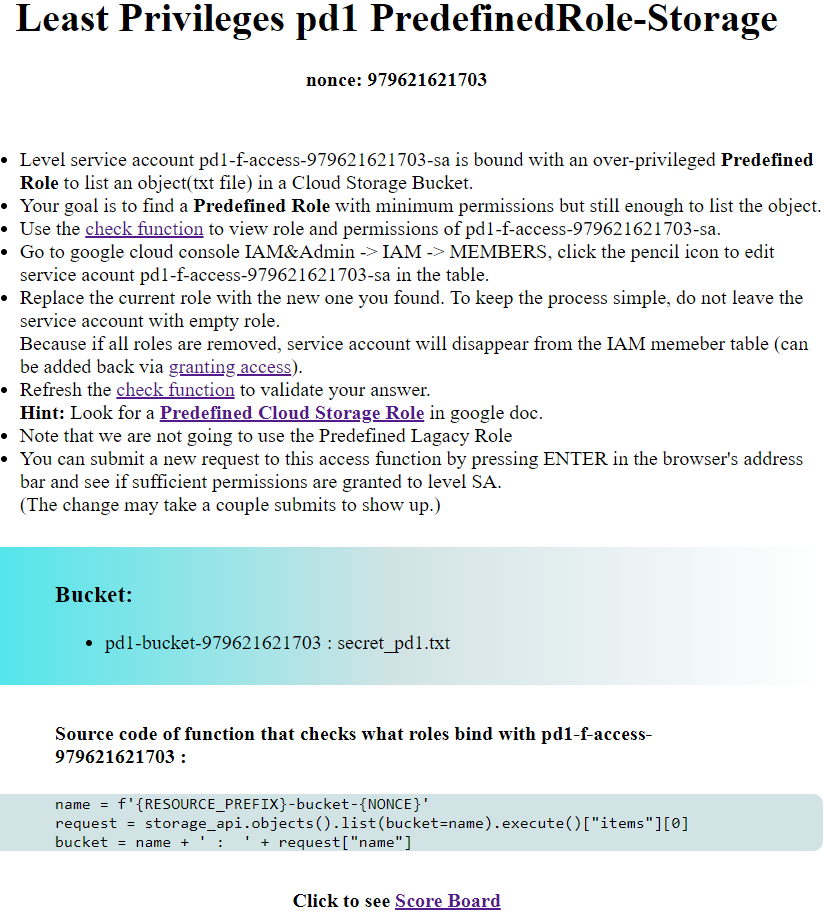
\includegraphics[width=0.5\textwidth]{pic/access}
  \caption {Access Function}
  \label{fig:access}
\end{figure}
\begin{figure}[!h]
  \centering
  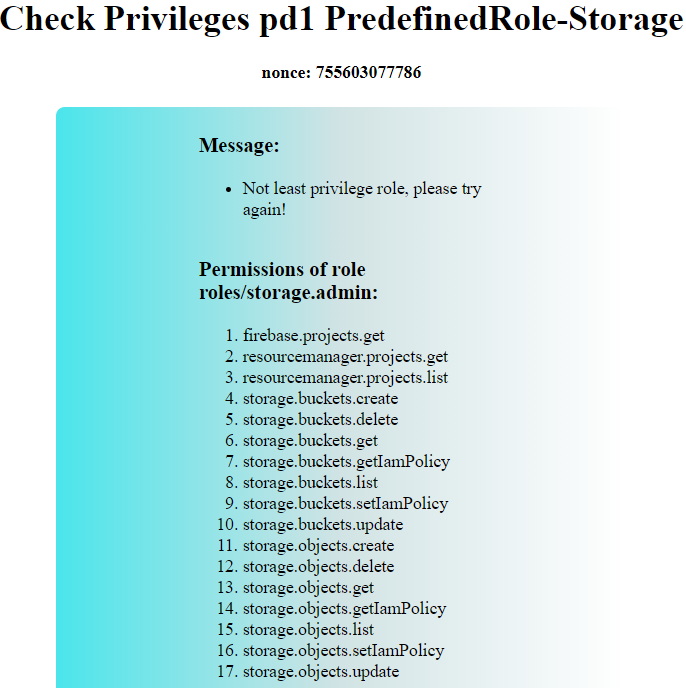
\includegraphics[width=0.5\textwidth]{pic/check}
  \caption {Check Function}
  \label{fig:check}
\end{figure}

\begin{figure}[!h]
  \centering
  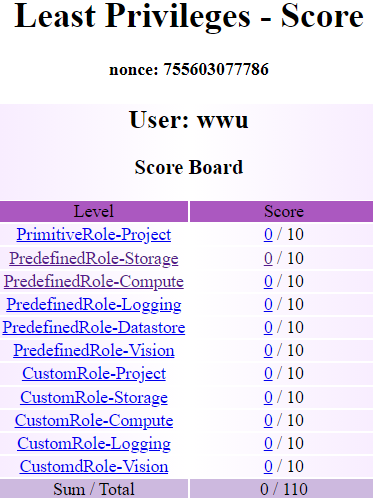
\includegraphics[width=0.4\textwidth]{pic/score}
  \caption {Scoreboard Function}
  \label{fig:score}
\end{figure}

\begin{figure*}[h]
  \centering
  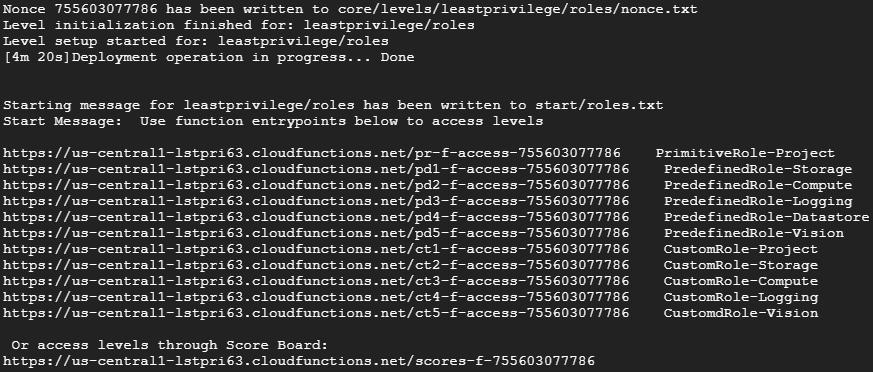
\includegraphics[width=0.7\textwidth]{pic/endpoints}
  \caption {Endpoints}
   \label{fig:endpoints}
\end{figure*}
%%\begin{figure*}[t]
%%  \centering
 %% \begin{tabular}{c}
 %% 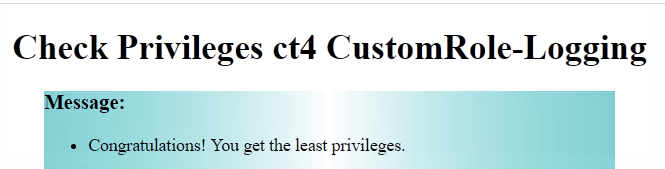
\includegraphics[width=0.60\textwidth]{success}
%%  \end{tabular}
%%\caption{Figure 1: function-validate answer and provide hints}
%%\label{fig:hints}
%%\end{figure*}
\subsubsection{Levels}
There are eleven levels implemented in Least Privilege CTF so far, and they are designed in a scaffolded style with incrementally increasing difficulties. The type of role and service that each level targets on are implied in level name and joined by a dash (first column of Figure~\ref{fig:score}). 

In the design of Least Privilege CTF, all functions are expected to access level resources only with their default identities, the service accounts created and attached during deployment. The roles bind with these service accounts can be updated after deployment in Google Cloud Console. 
A check function validates whether the binding role(s) in access function matche(s) the correct answer, so a role with permissions to list and get roles or IAM policy is always required. The score board function is using similar technique to validate answers and calculate scores, and repeat this for all levels. The roles bind with access functions are more complicated and vary based on specific levels. In general, access functions begin with a role of excessive permissions to perform certain actions described in level instruction. The winning condition is to apply PoLP and grant minimum privileges that are just enough to perform the same action. The process of picking and specifying more restrictive roles has been exemplified in Section~\ref{sec:gcpiam}.

Players may spend a little bit more time on the levels regarding Cloud Vision service - a service that does not have a set of predefined roles or permissions associated in GCP, indicating that the authenticated service accounts will have default access to Cloud Vision API. In order to analyse images with Cloud Vision service, the players are required to upload images into a Bucket through the form in front-end page (access function). The analysed results will be inserted into Cloud Datastore and listed in the same page.  The roles or permissions to complete such tasks are actually in Cloud Storage and Datastore category. The correct answer of level CustomRole-Vision is a combination of predefined role and custom role. As mentioned in Section~\ref{sec:gcpiam}, GCP does not support Datastore permissions in Custom Role yet.
 